\documentclass{i20lecture}

\subtitle{Session 0}
\usepackage{amssymb}

\newcommand{\done}{\makebox[0pt][l]{$\square$}\raisebox{.15ex}{\hspace{0.1em}$\checkmark$}}
\begin{document}

\frame{\titlepage}

%%%%%%%%%%%%%%%%%%%%%%%%%%%%%%%%%%%%%%%%%%%%%%%%%%%%%%%%%%%%%%%%%%%%%%%%%%%%%%%%%%%%%
\begin{frame}
  \frametitle{Timeline}

  \begin{center}
    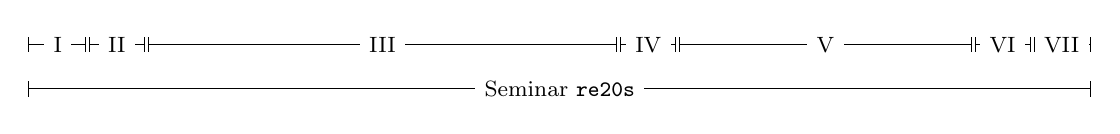
\begin{tikzpicture}[scale=.75]
      \path[|-|] (0, 0) edge node[pos=.5, fill=white] {\footnotesize Seminar \texttt{re20s}} (18, 0);
      \path[|-|, shorten > = .5pt, shorten < = .0pt, ] ( 0.00, 0.75) edge node[pos=.5, fill=white] {\footnotesize \alert{I}}    ( 1, 0.75);
      \path[|-|, shorten > = .5pt, shorten < = .5pt, ] ( 1.00, 0.75) edge node[pos=.5, fill=white] {\footnotesize \alert{II}}   ( 2, 0.75);
      \path[|-|, shorten > = .5pt, shorten < = .5pt, ] ( 2.00, 0.75) edge node[pos=.5, fill=white] {\footnotesize \alert{III}}  (10, 0.75);
      \path[|-|, shorten > = .5pt, shorten < = .5pt, ] (10.00, 0.75) edge node[pos=.5, fill=white] {\footnotesize \alert{IV}}   (11, 0.75);
      \path[|-|, shorten > = .5pt, shorten < = .5pt, ] (11.00, 0.75) edge node[pos=.5, fill=white] {\footnotesize \alert{V}}    (16, 0.75);
      \path[|-|, shorten > = .5pt, shorten < = .5pt, ] (16.00, 0.75) edge node[pos=.5, fill=white] {\footnotesize \alert{VI}}   (17, 0.75);
      \path[|-|, shorten > = .0pt, shorten < = .5pt, ] (17.00, 0.75) edge node[pos=.5, fill=white] {\footnotesize \alert{VII}}  (18, 0.75);
    \end{tikzpicture}
    \vfill
    \scalebox{.9}{
    \begin{tabular}{lp{4.9cm}ll}
      \toprule
      Phase       & Description             & Deliverable                          & Date \\
      \midrule
      \alert{I}   & Choose a topic          & --                             & \alert{22.04.2020} \\
  \alert{II}  & Surveying Literature    & Citation graph + Proposal (\emph{not} graded)                             & \alert{01.05.2020} \\
      \alert{III} & Writing / Experimenting & Paper Draft (\emph{not} graded)      & \alert{22.06.2020} \\
      \alert{IV}  & Reviewing               & Reviews of \emph{two} Seminar Papers & \alert{29.06.2020} \\
      \alert{V}   & Incorporating Suggestions + Writing / Experimenting
	                                        & Final Paper (``Camera Ready'')       & \alert{27.07.2020} \\
      \alert{VI}  & Preparing your Talk     & Final Slides                         & \alert{01.08.2020} \\
      \alert{VII} & Giving your Talk        & Final Talks                          & \alert{03.08.2020} / \\
      \alert{VIII} & ROOTS CFP               & -- (optional)                        & \alert{August 2020} \\
      \midrule
      --          & End of Lecture Period   & --                                   & \alert{07.08.2020} \\
      \bottomrule
    \end{tabular}
    }
  \end{center}
\end{frame}

\begin{frame}[fragile]
  \frametitle{Grading}
  \begin{tabular}{lrl}
             & \alert{40 \%}   & Final Paper (Content, Style, Language, Scope, \ldots)\\
             & \alert{15 \%}   & Experiments / Work on your tool \\
             & \alert{10 \%}   & Review      \\
             & \alert{30 \%}   & Presentation (Content, Style, Timeliness, \ldots) \\
             & \alert{5 \%}    & Discussion                                                   \\
    \midrule
	$\Sigma$ & \alert{100 \%}  & Total                                                        \\
  \end{tabular}
\end{frame}

\begin{frame}
  \frametitle{Orga}
  \begin{itemize}
	  \item Meeting (about) every \alert{2} weeks on BBB \alert{online}
	  \item Irregularly: Video-Tutorials done by \alert{us}
	  \item Regularly: Prepare \alert{0} - \alert{3} slides summarizing the last 2 weeks of
		  your work
	  \item Discuss progress, questions, problems, literature \dots
	  \item Collisions / problems?
  \end{itemize}
\end{frame}

\begin{frame}
	\frametitle{Topics}

	\begin{tabular}{lll}
		\textbf{Topic}                 & \textbf{Student} & \textbf{Contact person} \\\
		Build an Obfuscator on LLVM Framework                  & Justus     & Fabian \\
		SOK: Anti-Debugging Techniques used by Windows Malware & Arxhend    & Fabian \\
		Avatar² / Type propagation in Decomplilation            & Björn      & Fabian \\
		Hypervisor Detection                                   & Kevin      & Fabian \\
		SOK: Different Obfuscation Techniques                  & Benedikt K.& Ludwig \\
		WASM Decompiler                                        & Benedikt W.& Ludwig \\
		Code Virtualization                                    & Christian  & Ludwig \\
		Deobfuscation Control Flow Flattening                  & Maximilian & Ludwig \\
	\end{tabular}
\end{frame}

\begin{frame}[fragile]
	\frametitle{Next Tasks (due in two weeks!)}
  \begin{itemize}
	  \item Literature survey (for more details watch the \alert{video tutorial}!)
    \begin{itemize}
      \item \url{https://scholar.google.com}
      \item \url{https://semanticscholar.org}
	  \item \url{https://dblp.uni-trier.de}
      \item \url{https://arxiv.org}
      \item Get around paywalls using
          \url{https://login.eaccess.ub.tum.de/login} or bookmarklet:
          \begin{lstlisting}
javascript:void(location.href='https://eaccess.ub.tum.de/login?url='+location.href)
          \end{lstlisting}
      \item Researchers' homepages can be \alert{valuable}! (source code, raw data, instructions, technical information, ...)
    \end{itemize}
	\item Create a citation graph!
	\item Write a small proposal for your work (about half a A4 page)!
    %\item Practise your reversing skills on \texttt{\alert{challs.kirschju.re}}!
    %  (credentials in the repository)
  \end{itemize}
\end{frame}

\begin{frame}
	\frametitle{Citation graph} 

	\begin{center}
		\includegraphics[width=\linewidth]{citation_graph.png}
	\end{center}
\end{frame}

\begin{frame}
	\frametitle{The End (for today)}
	\begin{center}
		\Large Questions?
	\end{center}
\end{frame}

\end{document}
